\documentclass{article}

% if you need to pass options to natbib, use, e.g.:
%     \PassOptionsToPackage{numbers, compress}{natbib}
% before loading neurips_2026
\PassOptionsToPackage{numbers,compress}{natbib}

% The authors should use one of these tracks.
% Before accepting by the NeurIPS conference, select one of the options below.
% 0. "default" for submission
\usepackage[main, final]{neurips_2026}
\makeatletter
\renewcommand{\@noticestring}{}
\makeatother
% the "default" option is equal to the "main" option, which is used for the Main Track with double-blind reviewing.
% 1. "main" option is used for the Main Track
%  \usepackage[main]{neurips_2026}
% 2. "position" option is used for the Position Paper Track
%  \usepackage[position]{neurips_2026}
% 3. "eandd" option is used for the Evaluations & Datasets Track
 % \usepackage[eandd]{neurips_2026}
 % if you want to opt-in for a de-anomymized submission (not recommended, but OK):
 %\usepackage[eandd, nonanonymous]{neurips_2026}
% 4. "creativeai" option is used for the Creative AI Track
%  \usepackage[creativeai]{neurips_2026}
% 5. "sglblindworkshop" option is used for the Workshop with single-blind reviewing
 % \usepackage[sglblindworkshop]{neurips_2026}
% 6. "dblblindworkshop" option is used for the Workshop with double-blind reviewing
%  \usepackage[dblblindworkshop]{neurips_2026}

% After being accepted, the authors should add "final" behind the track to compile a camera-ready version.
% 1. Main Track
% \usepackage[main, final]{neurips_2026}
% 2. Position Paper Track
%  \usepackage[position, final]{neurips_2026}
% 3. Evaluations & Datasets Track
 % \usepackage[eandd, final]{neurips_2026}
% 4. Creative AI Track
%  \usepackage[creativeai, final]{neurips_2026}
% 5. Workshop with single-blind reviewing
%  \usepackage[sglblindworkshop, final]{neurips_2026}
% 6. Workshop with double-blind reviewing
%  \usepackage[dblblindworkshop, final]{neurips_2026}
% Note. For the workshop paper template, both \title{} and \workshoptitle{} are required, with the former indicating the paper title shown in the title and the latter indicating the workshop title displayed in the footnote.
% For workshops (5., 6.), the authors should add the name of the workshop, "\workshoptitle" command is used to set the workshop title.
% \workshoptitle{WORKSHOP TITLE}

% "preprint" option is used for arXiv or other preprint submissions
 % \usepackage[preprint]{neurips_2026}

% to avoid loading the natbib package, add option nonatbib:
%    \usepackage[nonatbib]{neurips_2026}

\usepackage[utf8]{inputenc} % allow utf-8 input
\usepackage[T1]{fontenc}    % use 8-bit T1 fonts
\usepackage{hyperref}       % hyperlinks
\usepackage{url}            % simple URL typesetting
\usepackage{booktabs}       % professional-quality tables
\usepackage{amsfonts}       % blackboard math symbols
\usepackage{nicefrac}       % compact symbols for 1/2, etc.
\usepackage{microtype}      % microtypography
\usepackage{xcolor}         % colors
\usepackage{microtype}
\usepackage{graphicx}
\usepackage{subcaption}
\usepackage{booktabs} % for professional tables
\usepackage{algorithm}
\usepackage{algpseudocode}
\usepackage{placeins}
\usepackage{booktabs}
\usepackage{amsmath}
% Note. For the workshop paper template, both \title{} and \workshoptitle{} are required, with the former indicating the paper title shown in the title and the latter indicating the workshop title displayed in the footnote. 
\title{Reproducing a DDPG-Based Stock Trading Strategy}


% The \author macro works with any number of authors. There are two commands
% used to separate the names and addresses of multiple authors: \And and \AND.
%
% Using \And between authors leaves it to LaTeX to determine where to break the
% lines. Using \AND forces a line break at that point. So, if LaTeX puts 3 of 4
% authors names on the first line, and the last on the second line, try using
% \AND instead of \And before the third author name.


\author{%
  George Kontorousis \\
  Department of Computer Science\\
  McGill University\\
  Montreal, Canada \\
  \texttt{george.kontorousis@mail.mcgill.ca} \\
  \And
  Yassine Meliani \\
  Department of Computer Science\\
  McGill University\\
  Montreal, Canada \\
  \texttt{yassine.meliani@mail.mcgill.ca} \\
}


\begin{document}


\maketitle


% Notes for abstract:
%  - The phrasing "Dow Jones data split" is not the best. Its actually the 30 stocks that the DJI tracks, and we use the same date ranges as the original paper. 
%  - We also did an additional experiment to evaluate how the DDPG and TD3 algorithms do for a different date range and "trade" phase on COVID-19 crash (for year of 2020) which showed that both DDPG and TD3 did not outperform the DJIA which indicate that these RL algorithms are not best when needing to adapt to crashes (possibly cause we did not train on a crash period?)
% also mention and change across the report actually that "TD3 showed higher mean performance than DDPG, albeit with increased variance, suggesting a potential advantage that requires further statistical confirmation."


\begin{abstract}
Stock trading is a challenging sequential decision-making problem because market dynamics are noisy and non-stationary. In this project, we reproduce the DDPG-based stock-trading formulation of \citet{liu2018practical}, where an agent observes cash, stock prices, and portfolio holdings, then learns buy, sell, and hold decisions to maximize portfolio value. Using the original Dow Jones data split, we compare DDPG and TD3 against DJIA and a min-variance portfolio allocation strategy as baselines. Both reinforcement learning agents outperform the min-variance baseline, while TD3 achieves the strongest final portfolio value and Sharpe ratio. We also run a COVID-19 stress test (train 2010--2019, trade 2020), where RL agents do not consistently outperform DJIA and min-variance, indicating sensitivity to volatile regime shifts.
\end{abstract}

\section{Background and Motivation}

Recent work has modeled stock trading as a Markov decision process, allowing reinforcement learning methods to optimize sequential trading decisions directly rather than relying on separate return forecasting and portfolio optimization stages \cite{liu2018practical}. In the target paper, Liu et al.\ formulate the trading state using current stock prices, portfolio holdings, and remaining cash balance, and train a Deep Deterministic Policy Gradient (DDPG) agent to maximize changes in portfolio value over time \cite{liu2018practical}. Their results show that this approach outperforms both the Dow Jones Industrial Average (DJIA) and a classical min-variance portfolio baseline in terms of cumulative return and Sharpe ratio \cite{liu2018practical}.

% maybe mention the date ranges that the original paper used
% also again the phrase "Dow Jones daily price data" is not the best
% 
% the point about 28 tradable stocks as opposed to 30 was also in the original paper code, due to missing entries in the csv file
This project reproduces that stock-trading reinforcement learning setup using the original Dow Jones daily-price data and the same train/validation/test split. After preprocessing, the dataset used in our environment contains 28 tradable stocks. The goal is to evaluate whether the main performance trend reported by Liu et al.\ can be recovered with a modern implementation pipeline, while also comparing DDPG against Twin Delayed Deep Deterministic Policy Gradient (TD3), a more stable actor-critic variant designed to reduce common sources of instability in deterministic policy-gradient methods \cite{fujimoto2018}.

% we do not propose a new trading algorithm; we reproduce the original paper, compare with TD3 and also do our own experiment for the covid 19 era (train from 2010-2019, trade on 2020)

% add references to the appendix about more details for the DIJA and especially the min-variance portfolio allocation strategy
% -- the original paper was referencing a broken url for the min-variance strategy they used so we just used a default one with PyPortfolioOpt (should mention in the appendix the details of the setup)
Rather than proposing a new trading algorithm, this work focuses on practical reproducibility and comparative evaluation. Financial reinforcement learning results are often sensitive to implementation details, hyperparameters, random seeds, and market dynamics, so we evaluate both learned agents against the same DJIA and min-variance baselines used in the original paper. Performance is measured using final portfolio value, annualized return, annualized volatility, and Sharpe ratio.


\section{MDP Formulation and State Space}

Following \cite{liu2018practical}, we model stock trading as a finite-horizon Markov decision process. At each trading day, the agent observes the current portfolio, chooses buy/sell/hold actions for each stock, and receives a reward equal to the change in total portfolio value. Since the environment uses a fixed historical price series, the transition is deterministic once the dataset split and action are fixed.

\begin{figure}[t]
    \centering
    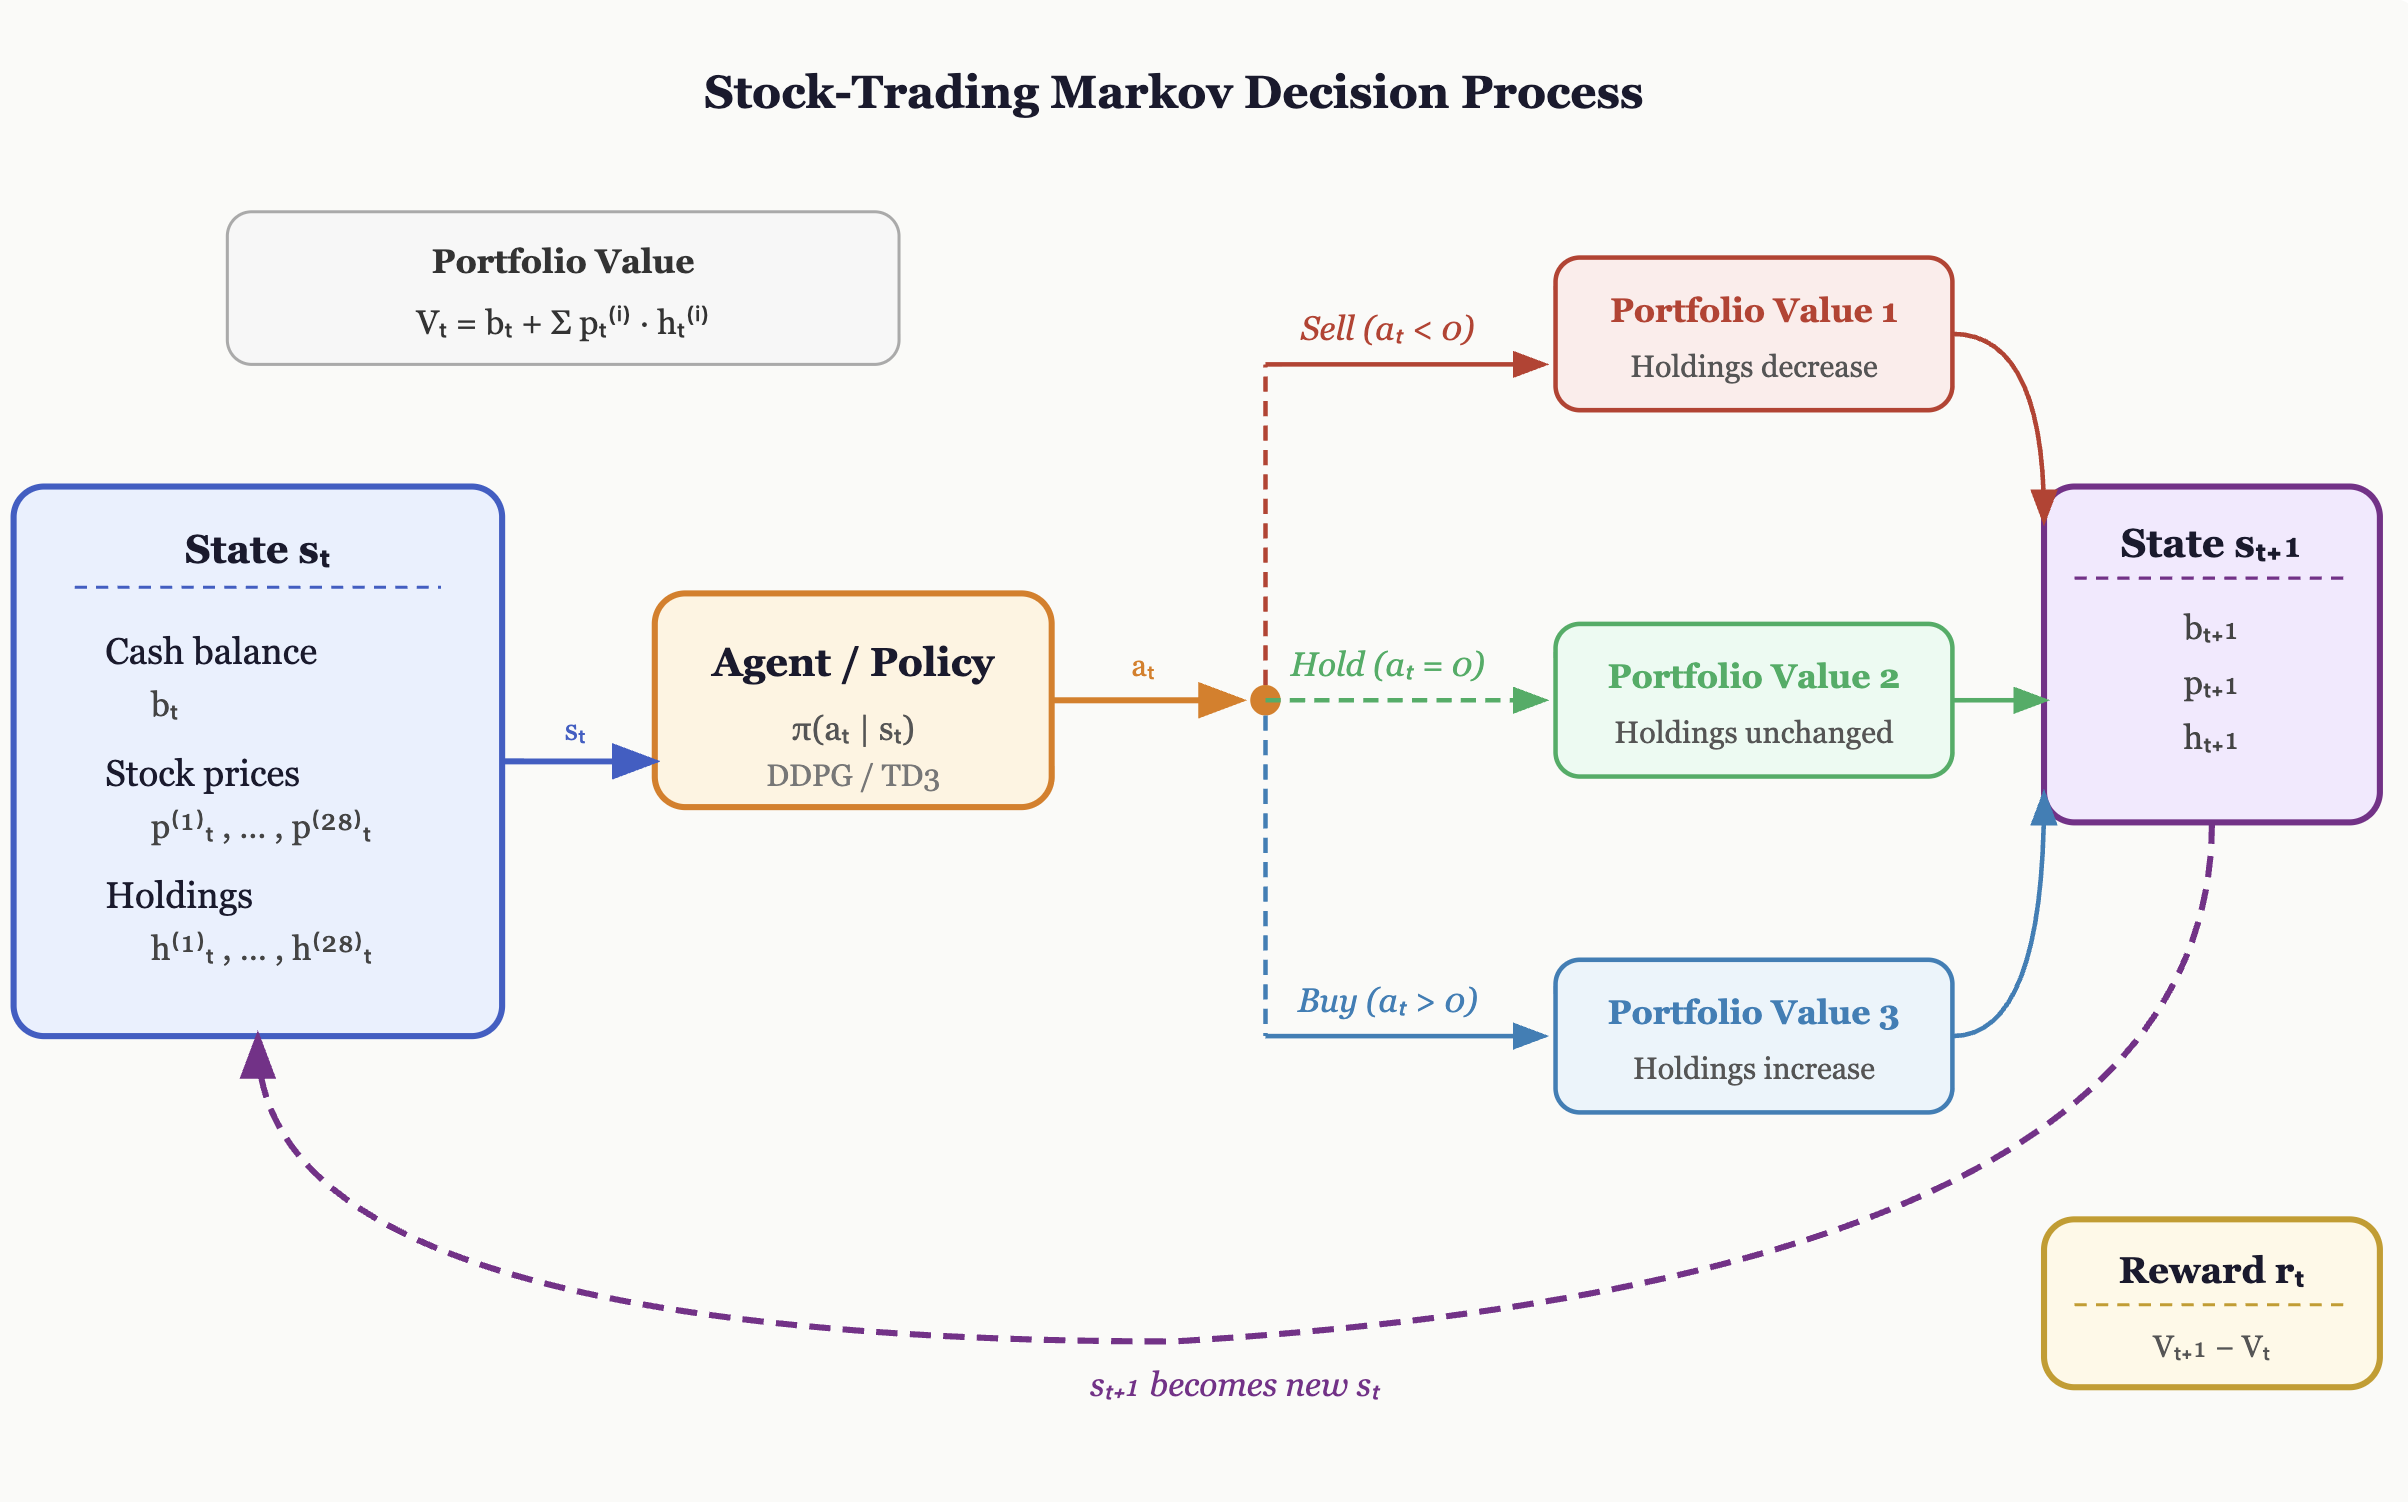
\includegraphics[width=0.95\linewidth]{resources/markov.png}
    \caption{Stock-trading MDP used in our reproduction. The agent observes cash, current prices, and current holdings, then selects bounded buy/sell actions. The environment executes trades, advances to the next trading day, and returns the change in portfolio value as the reward.}
    \label{fig:mdp_trading}
\end{figure}

The state contains cash, adjusted close prices, and holdings. Although the original paper refers to the Dow Jones 30 setting, our filtered dataset contains 28 tradable stocks, giving an observation vector of length 57:
\[
s_t =
\left[
b_t,
p_t^{(1)}, \ldots, p_t^{(28)},
h_t^{(1)}, \ldots, h_t^{(28)}
\right],
\]
where $b_t$ is cash, $p_t^{(i)}$ is the adjusted close price of stock $i$, and $h_t^{(i)}$ is the number of shares held. Each episode starts with \$10{,}000 in cash and zero holdings.

The action is a 28-dimensional trade vector,
\[
a_t =
\left[
a_t^{(1)}, \ldots, a_t^{(28)}
\right],
\]
with one action per stock. Actions are clipped, rounded, and executed as integers in
\[
a_t^{(i)} \in \{-5,-4,\ldots,0,\ldots,4,5\}.
\]
Negative values sell shares, positive values buy shares, and zero holds the position. The environment is long-only: holdings cannot become negative, and buy orders are limited by available cash. We do not model transaction costs, slippage, taxes, or borrowing.

The portfolio value is
\[
V_t = b_t + \sum_{i=1}^{28} p_t^{(i)} h_t^{(i)}.
\]
After the agent acts, the environment executes trades at the current day's prices, advances to the next trading day, and computes the reward as
\[
r_t = V_{t+1} - V_t.
\]

Thus, the agent is directly rewarded for increasing mark-to-market portfolio value. Each episode is one pass through a data split: training (2009--2014), validation (2015), or testing (2016--2018), which is also referred to as 'trading'. As in the original paper, policy updates continue during trading, so this is an online evaluation rather than a fixed-policy test. The episode ends at the final trading day of the given split.

\section{DDPG and TD3}

We evaluate two off-policy actor-critic methods for continuous control: DDPG \cite{lillicrap2015} and TD3 \cite{fujimoto2018}. In both methods, an actor maps the state to a continuous action and a critic estimates state-action value; replay buffers and target networks are used to stabilize training. This makes both algorithms suitable for our trading environment, where the policy outputs one value per stock before the environment converts actions into bounded integer buy/sell/hold decisions.

TD3 extends DDPG to improve stability by using twin critics (with a clipped double-Q target), delayed actor updates, and target policy smoothing. We include DDPG as the primary reproduced baseline from Liu et al.\ \cite{liu2018practical}, and TD3 as a stronger variant designed to reduce overestimation and noisy policy updates in this setting. Since DDPG and TD3 are well known algorithms, our discussion here is an overview of them; full algorithm outlines are provided in Appendix~\ref{app:algorithms}.

\section{Implementation}

We used the Stable-Baselines3 implementations of DDPG and TD3 \citep{stable-baselines3}, running both algorithms through the same training and evaluation pipeline. For both models, we reconstructed the original stock-trading task as a custom Gymnasium environment \citep{gymnasium}, using daily Yahoo Finance market data fetched with yfinance \citep{yfinance} for the Dow Jones constituent stocks over the selected training date range.

We performed Bayesian hyperparameter optimization with Optuna \citep{akiba2019optuna}, using 10 trials per algorithm. After selecting hyperparameters, each model was trained for 30 episodes and evaluated across three random seeds; results are reported as mean and standard deviation across seeds. Additional details about the hyperparameter tuning are provided in Appendix~\ref{app:hpo_details}.

%% may need to add more implementation details in main report?


\section{Results and Discussion}

Table~\ref{tab:trading_results} summarizes the final test-period performance of DDPG, TD3, the min-variance baseline, and the DJIA. Each reinforcement learning result is reported as the mean across three random seeds, with standard deviations shown in parentheses. Both RL agents outperformed the min-variance portfolio in final portfolio value and annualized return. DDPG slightly outperformed DJIA in annualized return while matching DJIA's Sharpe ratio. TD3 produced the strongest overall result, achieving the highest final portfolio value, annualized return, and Sharpe ratio; this higher Sharpe indicates better risk-adjusted performance. Representative portfolio-value curves from a specific seed are included in Appendix~\ref{app:portfolio_plots}; these show the same qualitative trend, with both learned agents tracking above the min-variance portfolio strategy baseline and TD3 ending above DDPG.


\begin{table}[H]
\centering
\caption{Trading performance on the 2016--2018 test period. RL results are reported as mean across seeds, with standard deviation in parentheses.}
\label{tab:trading_results}
\resizebox{\columnwidth}{!}{
\begin{tabular}{lcccc}
\toprule
Metric & DDPG & TD3 & Min-Variance & DJIA \\
\midrule
Initial Portfolio Value & \$10{,}000 & \$10{,}000 & \$10{,}000 & \$10{,}000 \\
Final Portfolio Value & \$16{,}141.47 $(630.95)$ & \$16{,}918.53 $(1002.53)$ & \$13{,}194.40 & \$15{,}594.84 \\
Annualized Return & 19.25\% $(1.73)$ & 21.31\% $(2.62)$ & 10.74\% & 17.76\% \\
Annualized Std. & 12.78\% $(0.99)$ & 12.67\% $(0.88)$ & 9.37\% & 11.74\% \\
Sharpe Ratio & 1.51 $(0.15)$ & 1.68 $(0.20)$ & 1.15 & 1.51 \\
\bottomrule
\end{tabular}
}
\end{table}

The main split partially reproduces Liu et al.\ \cite{liu2018practical}: both RL agents outperform the min-variance baseline, and TD3 is strongest overall. However, our DDPG result (\$16{,}141.47 final value) remains below the original reported value (\$19{,}791), likely because our training and hyperparameter search budget is smaller and the original tuning procedure is not fully specified.

TD3 improves over DDPG in mean final portfolio value (\$16{,}918.53 vs.\ \$16{,}141.47) and mean Sharpe ratio (1.68 vs.\ 1.51), consistent with its stabilizing design (twin critics, delayed policy updates, and target smoothing) \cite{fujimoto2018}. However, given the reported standard deviations (e.g., \$1002.53 vs.\ \$630.95 in final value), this advantage may be moderate rather than large. In this environment, where continuous actions are rounded into integer trades and rewards depend on noisy daily portfolio changes, these stabilizing changes likely helped TD3 produce better risk-adjusted returns on average. More broadly, the results suggest that future work should focus not only on more complex models, but also on more realistic and robust evaluation, including longer training budgets, broader hyperparameter searches, transaction costs, slippage, and evaluation across additional market periods.

We also ran an additional stress test using the best hyperparameters from the main reproduction, training for 500 episodes on 2010--2019 and trading on the volatile 2020 COVID period (same Dow Jones stock universe; setup details in Appendix~\ref{app:covid_setup}). In this regime, RL did not consistently outperform classical baselines: TD3 underperformed both DJIA and min-variance (final value \$9{,}785.69, Sharpe -0.04), while DDPG had only a small mean final-value edge (\$10{,}590.07 vs.\ DJIA \$10{,}533.71 and min-variance \$10{,}476.71) but high seed variance and weaker risk-adjusted performance than min-variance. This highlights sensitivity to regime shifts and questions the robustness of the original effectiveness claim under highly volatile markets.

\begin{table}[H]
\centering
\caption{COVID-19 stress-test performance on the 2020 trading period. RL results are mean across seeds, with standard deviation in parentheses.}
\label{tab:covid_results}
\resizebox{\columnwidth}{!}{
\begin{tabular}{lcccc}
\toprule
Metric & DDPG & TD3 & Min-Variance & DJIA \\
\midrule
Initial Portfolio Value & \$10{,}000 & \$10{,}000 & \$10{,}000 & \$10{,}000 \\
Final Portfolio Value & \$10{,}590.07 $(1261.53)$ & \$9{,}785.69 $(305.36)$ & \$10{,}476.71 & \$10{,}533.71 \\
Annualized Return & 5.93\% $(12.67)$ & -2.15\% $(3.07)$ & 4.79\% & 5.36\% \\
Annualized Std. & 40.87\% $(6.30)$ & 43.86\% $(6.03)$ & 23.87\% & 36.88\% \\
Sharpe Ratio & 0.18 $(0.32)$ & -0.04 $(0.07)$ & 0.20 & 0.15 \\
\bottomrule
\end{tabular}
}
\end{table}

\section{Conclusion}

We reproduced the stock-trading reinforcement learning setup of \cite{liu2018practical} using the same MDP formulation and historical Dow Jones data split. Our DDPG results followed the main trend of the original paper by outperforming the min-variance baseline, though they were weaker than the reported original results, likely due to a smaller training and hyperparameter-tuning budget and uncertainty around the original tuning procedure.

TD3 achieved the strongest performance in our experiments, outperforming DDPG in final portfolio value, annualized return, and Sharpe ratio. However, in an additional COVID-19 stress test on the volatile 2020 market, RL agents did not consistently outperform DJIA and min-variance baselines. Overall, these results suggest that while DDPG can learn useful trading behavior in this environment, TD3 provides a more stable and effective alternative for this reproduced stock-trading task, but robustness remains sensitive to market regime shifts.

\section*{Contributions and Acknowledgements}
Both authors contributed equally to the implementation, experiments, analysis, and writing. We thank the authors of the original stock-trading DDPG repository and the developers of Stable-Baselines3, Gymnasium, yfinance and Optuna for the tools used in this project.

\section{Code}
We make our code available in our GitHub repository. For the submission, we include here a link to the last commit that is dated before the deadline of May 1st 11:59pm. Here is the link for the commit \href{https://github.com/gkontorousis/COMP-579-Project/tree/64e5ef34394f66d59a6f273b9ea01abe5afedd4c}{64e5ef3}.


% In the unusual situation where you want a paper to appear in the
% references without citing it in the main text, use \nocite
\bibliographystyle{plainnat}
\bibliography{report}

%%%%%%%%%%%%%%%%%%%%%%%%%%%%%%%%%%%%%%%%%%%%%%%%%%%%%%%%%%%%%%%%%%%%%%%%%%%%%%%
%%%%%%%%%%%%%%%%%%%%%%%%%%%%%%%%%%%%%%%%%%%%%%%%%%%%%%%%%%%%%%%%%%%%%%%%%%%%%%%
% APPENDIX
%%%%%%%%%%%%%%%%%%%%%%%%%%%%%%%%%%%%%%%%%%%%%%%%%%%%%%%%%%%%%%%%%%%%%%%%%%%%%%%
%%%%%%%%%%%%%%%%%%%%%%%%%%%%%%%%%%%%%%%%%%%%%%%%%%%%%%%%%%%%%%%%%%%%%%%%%%%%%%%
\newpage
\appendix
% \onecolumn

\section{Portfolio Value Plots}
\label{app:portfolio_plots}
\FloatBarrier

\begin{figure}[h]
    \centering
    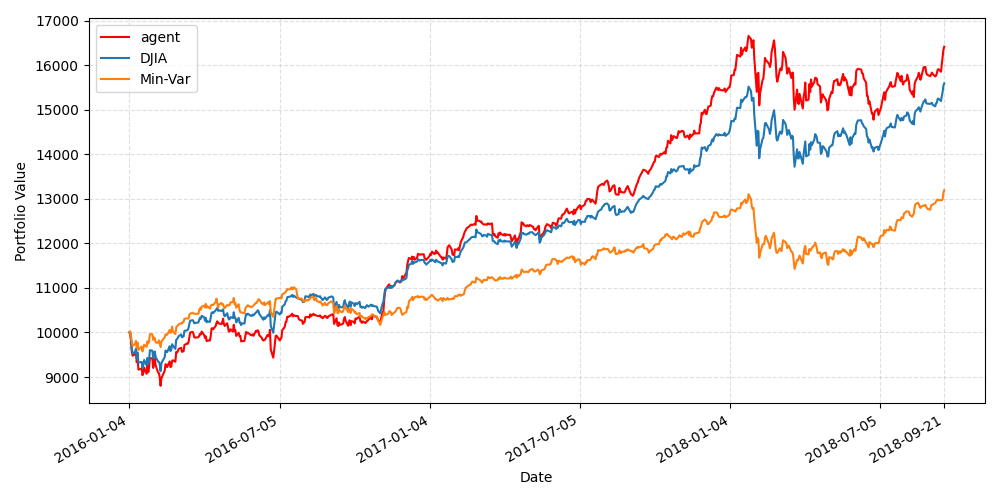
\includegraphics[width=0.95\linewidth]{resources/ddpg_model_test.png}
    \caption{DDPG portfolio value over the trading period compared against DJIA and the min-variance baseline. (seed 42)}
    \label{fig:ddpg_results}
\end{figure}

\begin{figure}[h]
    \centering
    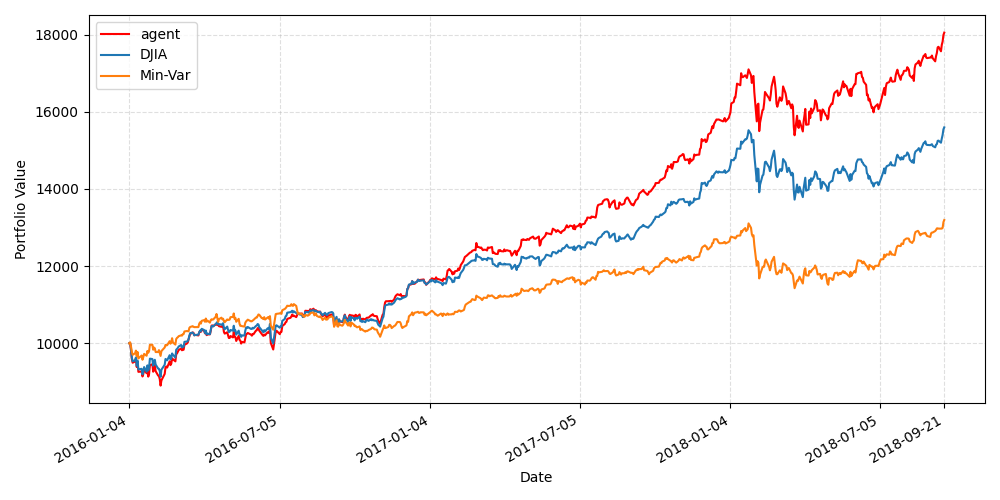
\includegraphics[width=0.95\linewidth]{resources/td3_model_test.png}
    \caption{TD3 portfolio value over the trading period compared against DJIA and the min-variance baseline. (seed 42)}
    \label{fig:td3_results}
\end{figure}

\FloatBarrier

\section{COVID-19 Stress-Test Setup and Results}
\label{app:covid_setup}
\FloatBarrier

We implemented the stress test in a similar pipeline as the main reproduction experiment. For each algorithm, we reused the best hyperparameters from the main reproduction (no re-tuning), then trained on 2010--2019 daily Dow Jones data and traded online on the 2020 COVID period, using the same Dow Jones universe, \$10{,}000 initial balance, and max 5 shares per trade (per ticker/stock). We evaluated three seeds (42, 43, 44), corresponding to 500 episodes (1{,}257{,}500 timesteps), and report mean and standard deviation across seeds for RL agents.

\FloatBarrier

\section{Hyperparameter Optimization Details}
\label{app:hpo_details}
\FloatBarrier

We tuned both DDPG and TD3 with Optuna over the same search ranges used in the implementation: learning rate in $[10^{-4}, 10^{-3}]$, batch size in $\{64,128,256\}$, discount factor $\gamma$ in $[0.95,0.999]$, soft-update rate $\tau$ in $[0.001,0.01]$, and exploration-noise scale $\sigma$ in $[0.05,0.3]$. For trial selection, we used Optuna's TPE sampler (\texttt{TPESampler}), which is a Bayesian hyperparameter optimization method.

Best hyperparameters from the 30-episode/10-trial main reproduction runs were:
\begin{itemize}
    \item \textbf{DDPG:} learning rate $= 3.6328 \times 10^{-4}$, batch size $=256$, $\gamma = 0.9533$, $\tau = 0.00568$, noise $\sigma = 0.21499$.
    \item \textbf{TD3:} learning rate $= 2.3150 \times 10^{-4}$, batch size $=64$, $\gamma = 0.96165$, $\tau = 0.00537$, noise $\sigma = 0.29054$.
\end{itemize}

\FloatBarrier

\section{Algorithm Details}
\label{app:algorithms}
\FloatBarrier

\begin{algorithm}[H]
\caption{DDPG}
\label{alg:ddpg}
\begin{algorithmic}[1]
\State Initialize actor network $\mu(s|\theta^\mu)$ and critic network $Q(s,a|\theta^Q)$
\State Initialize target networks $\mu'$ and $Q'$ with the same weights
\State Initialize replay buffer $\mathcal{R}$
\For{each episode}
    \State Receive initial state $s_1$
    \For{each time step $t$}
        \State Select action $a_t = \mu(s_t|\theta^\mu) + \mathcal{N}_t$
        \State Execute action $a_t$, observe reward $r_t$ and next state $s_{t+1}$
        \State Store transition $(s_t,a_t,r_t,s_{t+1})$ in $\mathcal{R}$
        \State Sample a mini-batch of transitions from $\mathcal{R}$
        \State Compute target:
        \[
        y_i = r_i + \gamma Q'(s_{i+1}, \mu'(s_{i+1}))
        \]
        \State Update critic by minimizing:
        \[
        L = \frac{1}{N}\sum_i \left(y_i - Q(s_i,a_i)\right)^2
        \]
        \State Update actor using the policy gradient:
        \[
        \nabla_{\theta^\mu}J \approx
        \frac{1}{N}\sum_i
        \nabla_a Q(s,a)|_{s=s_i,a=\mu(s_i)}
        \nabla_{\theta^\mu}\mu(s_i)
        \]
        \State Soft-update target networks:
        \[
        \theta^{Q'} \leftarrow \tau \theta^Q + (1-\tau)\theta^{Q'},
        \qquad
        \theta^{\mu'} \leftarrow \tau \theta^\mu + (1-\tau)\theta^{\mu'}
        \]
    \EndFor
\EndFor
\end{algorithmic}
\end{algorithm}

\begin{algorithm}[t]
\caption{TD3}
\label{alg:td3}
\begin{algorithmic}[1]
\State Initialize actor network $\mu(s|\theta^\mu)$
\State Initialize two critic networks $Q_1(s,a|\theta^{Q_1})$ and $Q_2(s,a|\theta^{Q_2})$
\State Initialize target networks $\mu'$, $Q'_1$, and $Q'_2$
\State Initialize replay buffer $\mathcal{R}$
\For{each episode}
    \State Receive initial state $s_1$
    \For{each time step $t$}
        \State Select action $a_t = \mu(s_t|\theta^\mu) + \mathcal{N}_t$
        \State Execute action $a_t$, observe reward $r_t$ and next state $s_{t+1}$
        \State Store transition $(s_t,a_t,r_t,s_{t+1})$ in $\mathcal{R}$
        \State Sample a mini-batch of transitions from $\mathcal{R}$
        \State Add clipped noise to the target action:
        \[
        \tilde{a}_{i+1} = \mu'(s_{i+1}) + \epsilon,
        \qquad
        \epsilon \sim \mathrm{clip}(\mathcal{N}(0,\sigma), -c, c)
        \]
        \State Compute target using the smaller critic value:
        \[
        y_i = r_i + \gamma \min_{j=1,2} Q'_j(s_{i+1}, \tilde{a}_{i+1})
        \]
        \State Update both critics by minimizing:
        \[
        L_j = \frac{1}{N}\sum_i \left(y_i - Q_j(s_i,a_i)\right)^2,
        \qquad j \in \{1,2\}
        \]
        \If{policy update step}
            \State Update actor using $Q_1$:
            \[
            \nabla_{\theta^\mu}J \approx
            \frac{1}{N}\sum_i
            \nabla_a Q_1(s,a)|_{s=s_i,a=\mu(s_i)}
            \nabla_{\theta^\mu}\mu(s_i)
            \]
            \State Soft-update target networks
        \EndIf
    \EndFor
\EndFor
\end{algorithmic}
\end{algorithm}



%%%%%%%%%%%%%%%%%%%%%%%%%%%%%%%%%%%%%%%%%%%%%%%%%%%%%%%%%%%%%%%%%%%%%%%%%%%%%%%
%%%%%%%%%%%%%%%%%%%%%%%%%%%%%%%%%%%%%%%%%%%%%%%%%%%%%%%%%%%%%%%%%%%%%%%%%%%%%%%

\end{document}

\newpage
\input{checklist.tex}


\end{document}